% A pesquisa de dados estatísticos foi conduzida por meio de um formulário composto por cinco questões, o qual foi respondido por cinco profissionais da área da Psicologia. No que se refere aos estímulos visuais empregados para a detecção de indícios de desatenção em crianças, os participantes destacaram que fatores como foco, tempo, som, cores e movimento constituem parâmetros relevantes para essa finalidade. Em virtude dessas considerações, tais elementos foram incorporados em todas as etapas do jogo desenvolvido. Ademais, todos os profissionais consultados reconheceram o rastreamento ocular como uma ferramenta útil, indicando que sua aplicação no contexto da abordagem proposta apresenta potencial para contribuir de forma eficaz na identificação de comportamentos relacionados à desatenção. Por fim, foram registradas sugestões de aprimoramento metodológico, como redirecionar o foco do estudo para uma aplicação de caráter clínico, inserir uma fase com estímulos \textit{distractors}, seguida de questionamentos específicos sobre o conteúdo \textit{distractor}, bem como assegurar que os estímulos sejam facilmente reconhecíveis pelas crianças participantes.

A \textit{landing page} do projeto foi desenvolvida em \textit{HTML}, responsável pela estrutura do conteúdo, \textit{CSS}, utilizado para o estilo visual, e \textit{JavaScript}, empregado na implementação da interatividade e do dinamismo da navegação. O sistema de rastreamento ocular foi implementado em JavaScript, utilizando a biblioteca \textit{WebGazer.js}, que contém um modelo capaz de se autocalibrar ao observar a interação dos visitantes com a página, treinando um mapeamento entre as características do olhar e as posições na tela \cite{papoutsaki2016webgazer}. O tratamento das coordenadas oculares recebidas do \textit{frontend} foi realizado em JavaScript, com o uso do \textit{Node.js} e do \textit{Socket.IO}, possibilitando a comunicação em tempo real com o frontend, uma vez que depende das coordenadas enviadas por ele. Essa parte do \textit{backend} é responsável por analisar as métricas TDC (acertos e erros), dados que serão utilizados para compor o feedback individual de cada usuário. Por fim, o jogo \textit{web} foi desenvolvido em \textit{TypeScript}, utilizando o \textit{framework} \textit{Next.js}, o que proporcionou um código mais robusto, organizado e uma experiência de uso moderna e fluida.

A metodologia fundamenta-se na aplicação adaptada do TDC. A principal diferença do presente trabalho está na integração do teste com o rastreamento ocular em tempo real, permitindo a coleta de dados visuais complementares durante a execução das tarefas.

O experimento é estruturado como um jogo digital de temática espacial, composto por
três fases com níveis crescentes de dificuldade. A mecânica de jogo foi desenhada para simular os
princípios do TDC, promovendo a exposição contínua a estímulos visuais por períodos prolongados e exigindo respostas rápidas e consistentes por parte do participante. Ao longo de cada fase, o sistema registra métricas relacionadas à atenção, como erros de omissão (quando o participante não responde a um estímulo-alvo), erros de comissão (quando não mantém foco por tempo suficiente no alvo), tempo de reação e variabilidade temporal das respostas. COLOCAR REF

Durante toda a experiência, o rastreamento ocular é realizado em segundo plano, utilizando a biblioteca WebGazer para capturar os pontos de fixação visual do usuário por meio da \textit{webcam}. Esses dados permitem identificar padrões de atenção ou desatenção de acordo com nossa base de dados em cada etapa da atividade. Todas as fases contam com música de fundo, cuja intensidade e ritmo são ajustados conforme o nível de dificuldade, de forma a potencializar a sobrecarga sensorial e dificultar a concentração.

Após o realizar login, o participante é direcionado para a página de instruções, onde são apresentadas a sequência de como calibrar o olhar para poder prosseguir para o jogo. Antes de cada fase, exitem as instruções da própria fase. Em seguida, o usuário inicia a primeira fase do teste. 

\begin{figure}[H]
    \centering
    \caption{Primeira fase}%
    \label{fig:primeira-fase}
    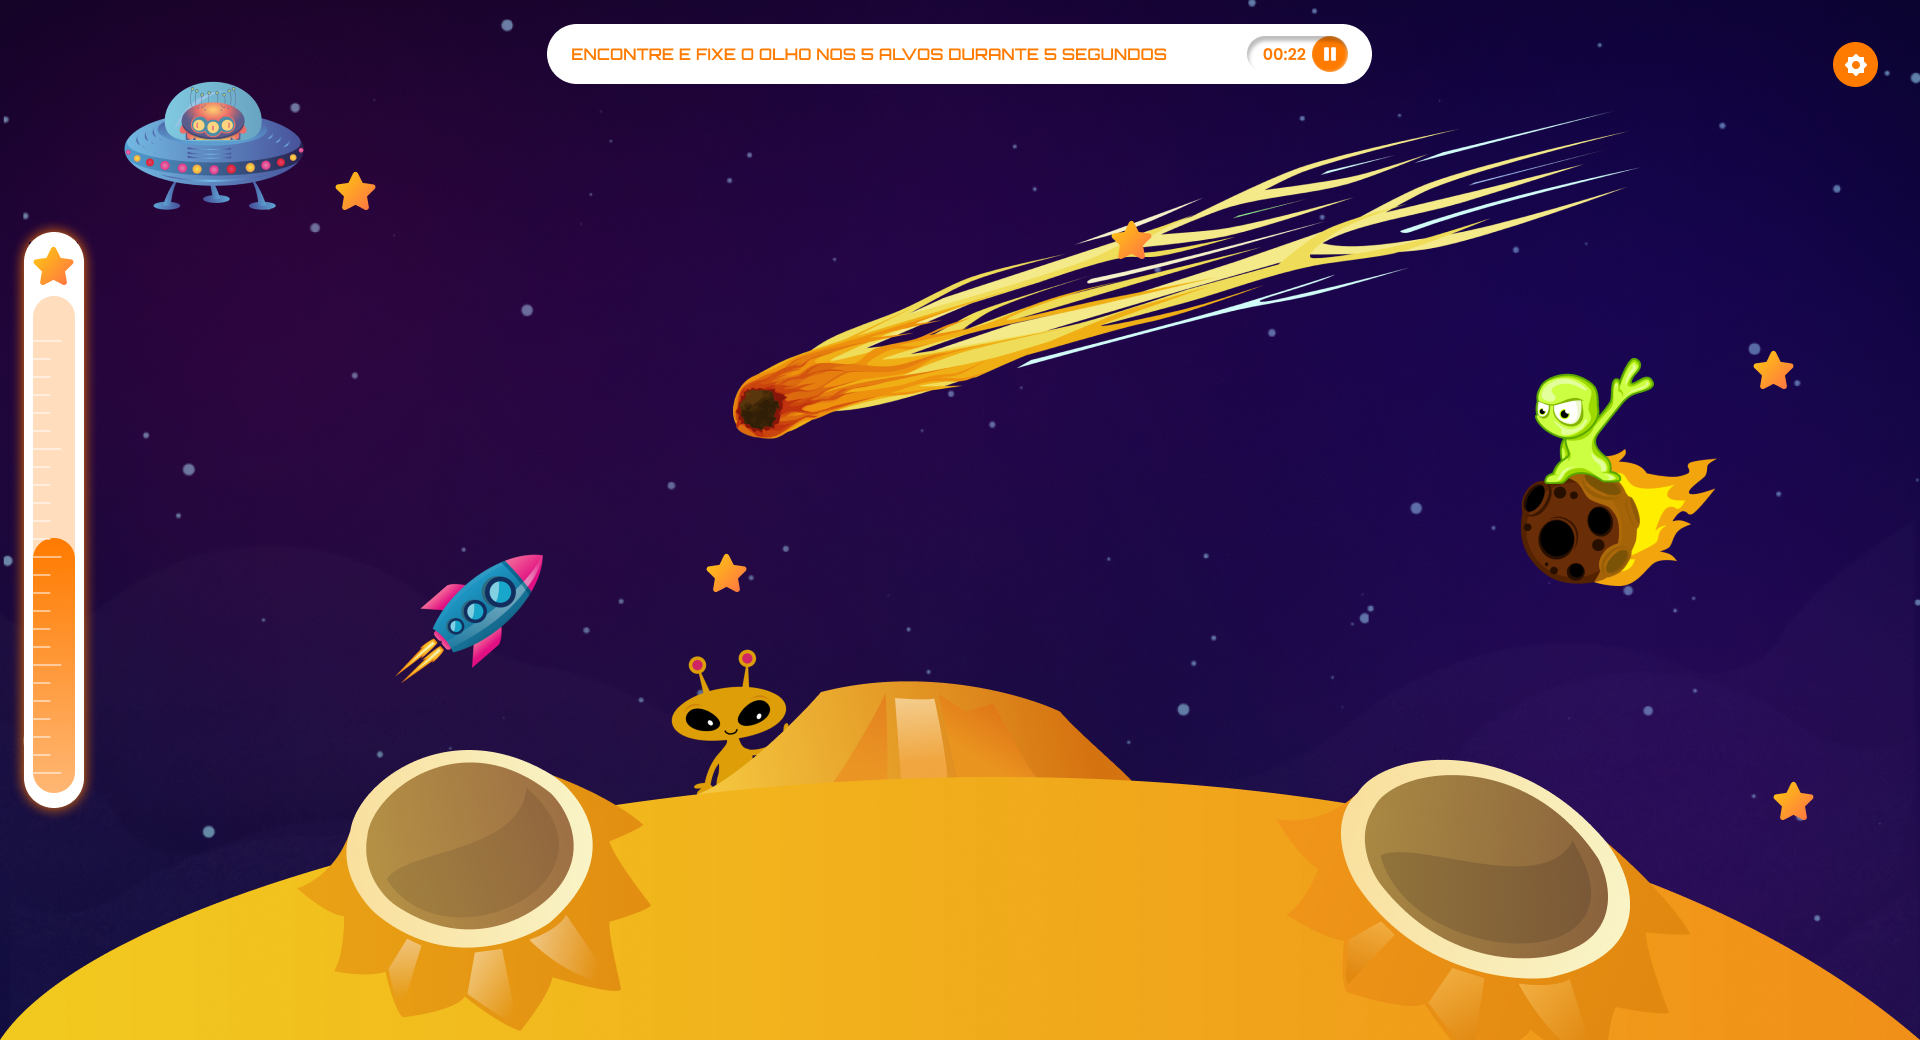
\includegraphics[width=\textwidth]{primeira-fase.png}%
    \SourceOrNote{Autoria Própria (2025)}
\end{figure}

Na primeira fase, o participante deve fixar o olhar por cinco segundos em cinco alvos estáticos,
representados por estrelas, enquanto elementos animados surgem ao redor. Após os 5 segundos,
cada estrela desaparece da tela. A música de fundo nesta etapa apresenta um ritmo moderado. O
objetivo é avaliar a capacidade de manter a atenção em um ponto fixo durante um tempo determinado, ignorando estímulos visuais e auditivos periféricos.

\begin{figure}[H]
    \centering
    \caption{Segunda fase}%
    \label{fig:segunda-fase}
    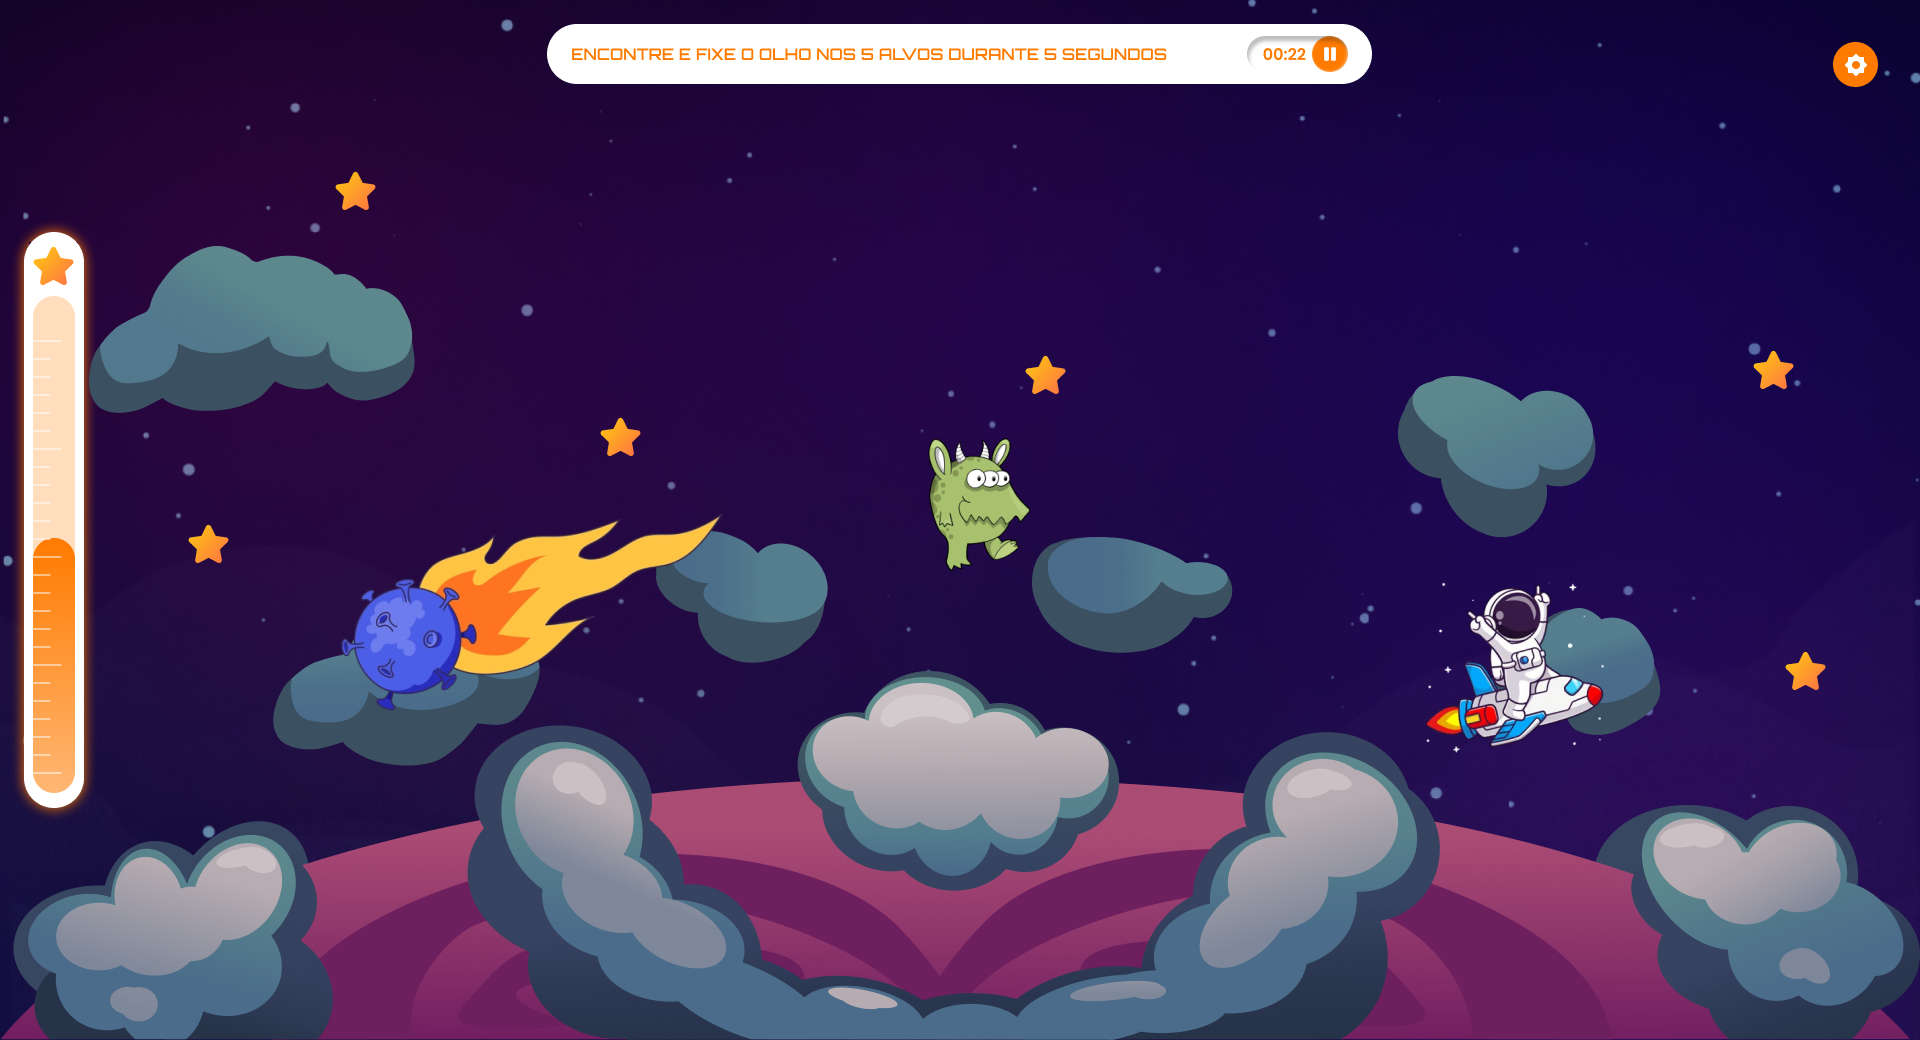
\includegraphics[width=\textwidth]{segunda-fase.png}%
    \SourceOrNote{Autoria Própria (2025)}
\end{figure}

Na segunda fase, são apresentadas cinco estrelas estáticas que brilham individualmente em sequência. Simultaneamente, três planetas transitam pela tela, atuando como estímulos secundários que o participante deve reconhecer. Ao término desta fase, o usuário responde a um formulário utilizando botões IoT, cada um correspondente a um planeta específico. O objetivo é que o participante aperte o botão do planeta X se, e somente se, o tiver observado em trânsito. Essa etapa visa mensurar a capacidade de identificar alvos dinâmicos (os planetas) enquanto o participante mantém o foco em estímulos estáticos (as estrelas). A trilha sonora, que se torna mais intensa e acelerada, tem o propósito de aumentar o nível de exigência atencional e avaliar a concentração diante de múltiplos estímulos visuais e auditivos.

Para a construção do dispositivo de controle da IoT, foram empregados os seguintes componentes eletrônicos: uma placa de desenvolvimento Arduino, três botões do tipo push-button, três resistores de 10 k$\Omega$, uma protoboard e cabos de conexão. Os botões foram conectados às portas digitais do Arduino, configuradas como entradas com resistores pull-down para garantir leituras estáveis [COMPLEMENTAR MAIS QUANDO ESTIVER PRONTO]. Dessa forma, ao término da segunda fase do jogo, o participante registra os planetas que conseguiu observar, pressionando o botão correspondente a ele. [COLOCAR BOTÃO 1 É DE SATURNO, POR EXEMPLO]. O Arduino foi programado para detectar os eventos de pressionamento dos botões e enviar os dados correspondentes ao backend do sistema por meio de comunicação serial. Essa comunicação permite o registro e a contabilização das respostas do participante durante a referida fase do jogo. Em futuras iterações do projeto, planeja-se o aperfeiçoamento estético e ergonômico do controle, por meio da substituição dos botões convencionais por peças personalizadas, modeladas em software CAD e fabricadas via impressão 3D, com design mais atrativo e ergonômico para crianças. Além disso, planeja-se construir uma case para o controle utilizando filamentos de plástico biodegradável [NÃO É ESSE O NOME, VER COM FREDERICO], visando a sustentabilidade ambiental do projeto.

\begin{figure}[H]
    \centering
    \caption{Terceira fase}%
    \label{fig:terceira-fase}
    \SourceOrNote{Autoria Própria (2025)}
\end{figure}

Na terceira fase, a demanda cognitiva é intensificada pela necessidade de alternância rápida do foco visual entre diferentes regiões da tela, caracterizadas por menor previsibilidade espacial. Nessa etapa, uma estrela surge de forma estática, exigindo resposta ocular imediata do participante. Simultaneamente, um segundo estímulo estático é apresentado, alternando entre os estados ligado e desligado em intervalos regulares. Quando esse estímulo é ativado (ascende), o participante deve manter o olhar fixo sobre ele até que se apague, o que permite avaliar a atenção sustentada e o controle do direcionamento ocular. A trilha sonora atinge seu nível máximo de intensidade e agitação, contribuindo para aumentar a complexidade da tarefa. O desempenho do participante nesta fase é utilizado como indicador da agilidade atencional e da capacidade de redirecionamento e manutenção do foco visual diante de estímulos dinâmicos.

Ao término das três fases, o sistema apresenta ao participante um resumo dos resultados com base nas métricasa TDC. Para isso, são utilizados os três registros mais recentes de rastreamento ocular, que correspondem às três fases concluídas pelo jogador. Com base nesses dados, o sistema gera um feedback textual interpretativo, apresentando mensagens como: “Sua atenção está conforme o esperado”, “Sua atenção está acima do esperado” ou “Sua atenção está abaixo do esperado.”, de acordo com o desempenho observado.

A plataforma é desenvolvida com tecnologias \textit{web}, permitindo acesso remoto e execução
direta em \textit{browsers} modernos. O teste é realizado de forma autônoma pelo usuário, em ambiente silencioso e seguindo instruções fornecidas pela própria plataforma.

No projeto atual, IA será utilizada para comparar os dados coletados durante o jogo, referentes aos erros e acertos, com uma base de dados previamente formada por indivíduos diagnosticados com TDA e por outros sem o transtorno. Entretanto, nesta fase inicial de desenvolvimento, é necessário testar a viabilidade do sistema. Inicialmente, dez crianças com TDA serão convidadas a participar do experimento, com o objetivo de coletar dados iniciais que servirão como base para o treinamento do modelo de IA. Em seguida, três crianças com TDA e três sem o transtorno (não podem ser as dez iniciais) 
serão convidadas para uma nova etapa experimental, destinada a validar a eficácia do sistema na identificação de indícios de desatenção. O objetivo é garantir que a acurácia do sistema seja satisfatória antes de ampliar a base de dados e aperfeiçoar o modelo de IA. Após a conclusão da fase de validação, o sistema estará apto a ser utilizado por um público mais amplo, contribuindo para a identificação precoce do TDA em crianças e reforçando seu potencial como ferramenta de apoio ao diagnóstico. 

No que se refere à retroalimentação da IA, o sistema dispõe de um modo de treinamento, que pode ser ativado ou desativado exclusivamente pelo administrador. A mecânica dessa funcionalidade é empregada sempre que houver necessidade de alimentar a base de dados com novos registros. Essa etapa só pode ser executada na presença de ao menos um administrador, a fim de garantir a integridade e a qualidade dos dados inseridos. Caso contrário, a criança participa normalmente do jogo apenas para avaliar seu nível de atenção. Quando o modo de treinamento está habilitado, o sistema armazena as métricas TDC coletadas durante as partidas em uma base de dados, permitindo que o módulo de treinamento da IA realize a análise comparativa entre os dados do indivíduo e a base existente. Esse processo tem como objetivo retroalimentar o modelo e aperfeiçoar continuamente o desempenho da IA. 

Para uma melhor compreensão do funcionamento do sistema, a Figura \ref{fig:fluxograma} apresenta o fluxograma do processo, que descreve a sequência lógica das operações realizadas pelo sistema até o término das três partidas. Na etapa 1, ocorre a calibração dos olhos do jogador, processo em que o sistema identifica e ajusta os pontos de fixação ocular do usuário antes do início do jogo, garantindo a precisão do rastreamento. Em seguida, é executada a coleta das métricas TDC, que ocorre automaticamente durante as três fases do jogo. Nessa etapa, o sistema processa e registra parâmetros como número de acertos, erros de omissão, erros de comissão, tempo de reação e variabilidade temporal das respostas. Concluída a coleta, o sistema entra em um ponto de decisão para verificar o modo de execução selecionado. Na etapa 2, há uma tomada de decisão para verificar se o participante irá jogar no modo de treinamento. Caso o modo de treinamento esteja habilitado (etapa 3), o sistema armazena as métricas TDC em uma base de dados, permitindo que o módulo de treinamento da IA realize a análise comparativa entre os dados do indivíduo e a base existente. Esse processo visa aprimorar o modelo e gerar um pré-diagnóstico personalizado. Já na etapa 4, quando o modo de treinamento não está ativado, o sistema realiza diretamente a geração e exibição do pré-diagnóstico, utilizando as métricas coletadas durante a execução do jogo.

\begin{figure}[H]
    \centering
    \caption{Fluxograma do sistema}%
    \label{fig:fluxograma}
    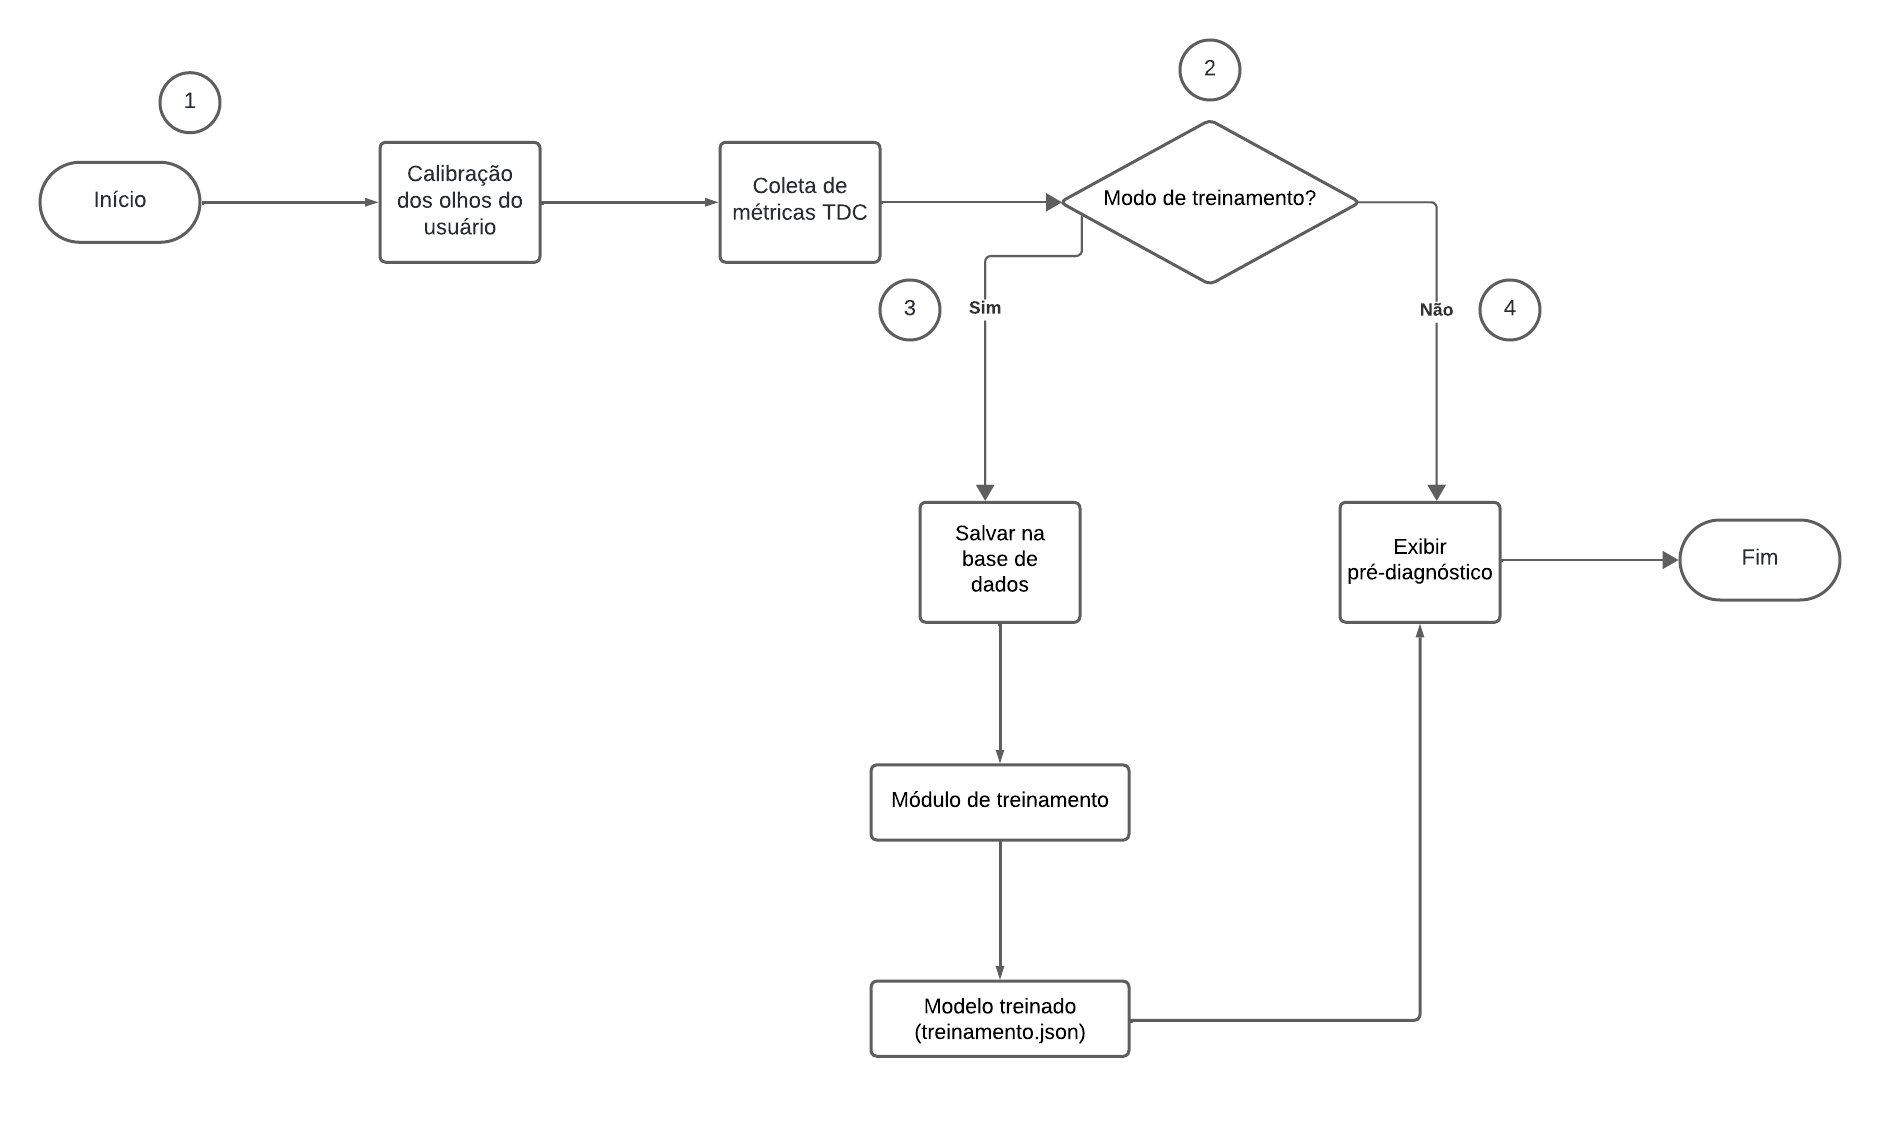
\includegraphics[width=\textwidth]{fluxograma.png}%
    \SourceOrNote{Autoria Própria (2025)}
\end{figure}

Optou-se pela utilização do banco de dados não relacional \textit{MongoDB}, o qual armazena informações em documentos no formato \textit{JSON}, possibilitando a criação de estruturas dinâmicas e aninhadas, adequadas ao armazenamento dos dados provenientes dos testes de rastreamento ocular. Sua flexibilidade e escalabilidade o tornam mais apropriado que bancos relacionais para o tratamento de grandes volumes de dados sensoriais. O gerenciamento do banco foi realizado por meio do \textit{MongoDB Compass}, ferramenta que facilita a execução de consultas, validação de esquemas e análise de desempenho.
